\chapter{Integration in a Neo4j}

In this section it is described how "Customizable Contraction Hierarchies" CCH is integrated into Neo4j. CCH arguments the input graph, which means it inserts arcs, so called shortcuts, that do not belong to the original data. To keep the change to the input graphs as little as possible we decided to not insert any arc into the graph that is stored inside the neo4j database, but introduce another graph data structure, the index graph. 
The mapping between the index and the graph that resides in the database is achieved by the rank property. The rank property is set to the input and the the index graph at contraction time. Through this we achieve a unique mapping between $G$ and $G'$.
This gives yet another two advantages. One is that we get full control about the graph representation which is helpful to efficiently store and read the index graph for the disk. Another is that the with this approach it makes it easier to later on port the idea to another graph database manufactures.

\section{Index Graph Data Structure}\label{sec:index_graph}

\begin{figure}
    \begin{tikzpicture}
    \begin{class}[text width=0.5\linewidth]{Vertex}{0,0}
        \attribute{+ rank : int}
        \attribute{+ inArcs : Map<Vertex, Arc>}
        \attribute{+ outArc : Map<Vertex, Arc>}
        \operation{+ Vertex(rank: int)}
        \operation{+ addArc(other: Vertex, middle: Vertex, weight: int, hopLength:int) }
      \end{class}
\end{tikzpicture} 
    \begin{tikzpicture}
    \begin{class}[text width=0.5\linewidth]{Arc}{0.5\linewidth, 0}
      \attribute{+ start : Vertex}
      \attribute{+ end : Vertex}
      \attribute{+ middle : Vertex}
      \attribute{+ weight : int}
      \attribute{+ hopLength: int}
      \operation{+ Arc(start: Vertex, end: Vertex, weight: int, middle: Vertex, hopLength: int) }
      \operation{+ other(vertex: Vertex): Vertex}
    \end{class}
\end{tikzpicture}
    \caption{Index Graph}
    \label{uml:index_graph}
\end{figure}

The index graph data structure is neither a adjacency list nor adjacency matrix. There is a vertex object that has two hash tables. One for incoming arc and one for outgoing arcs. The hash tables keys are of type vertex and the value is the arc. An arc has a reference to its start vertex and one to its end vertex. \\
A disadvantage of this model could be that some modern hardware optimization that exist for arrays do not match with this data structure. Due to paging algorithms as described in \cite[Modern Operatins Systems]{andrew2015modern} when using an array, the values this array are stored sequentially in main memory. When one value of an array is accessed by the CPU, modern hardware reads subsequent values into the CPU-cache because it is likely that they are accessed right after it. The model of the index graph is a linked data structure, a bit like a linked list. The elements of an linked list are contained somewhere in main memory. There is no guarantee that subsequent values have any spacial proximity. Therefore the just explained hardware optimization will not apply. \\ % cite some paper to this topic
However, this makes the the graph traversal easy. Additional it makes it very efficient to explore the neighborhood of a vertex. There is no array traversal to find a vertex and only one hash table lookup for finding an arc of a vertex. Additionally these hash tables only contain few elements. Test on small graphs [Oldenburg] show that cch queries can be answered in less than one millisecond, which is close to what we tested with the original cch application.

\section{The Mapping}\label{sec:mapping}

The in memory data structure of neo4j is similar to the just explained index graph data structure in section \ref{sec:index_graph}. A \textit{node} has a collection of \textit{relationships} and a \textit{relationship} has a reference to its \textit{start node} and \textit{end node}.
As neo4j is a full blown property graph nodes and relationship contain a lot of other information. A node has a collection of \textit{labels}, relationship has a \textit{type}. The class \textit{Node} and the class \textit{Relationship} 
are both derived from the class \textit{Entity} which also has a collection of properties as well as and id that is managed by the database system. Note that, as of version Neo4j 5.X, this id can change over time and should not be used to make mappings to external systems. Additionally 
worth to mentioning here is that the Neo4j system shifted its id concept as it moved from major release 4 to 5. Until major release 4 every entity had a unique integer identifier. Since major release 5 every entity has a string identifier which is a UUID and the old \textit{id} identifier
isn't guaranteed to be unique anymore. It is deprecated and marked for removal.
\\
As just explained there are lot of information in this data structure. A lot of information we don't need. Looking at \ref{fig:mapping} we only want to keep track of the information that is needed for the CCH index. Additionally as disks are
divided  into blocks and sectors we want to flatten the graph which is in memory more looks like a tree to a structure that looks like a table. Therefore we decided that the disk data structure only consists of edges $\bigcirc A$. A disk edge $a \epsilon \bigcirc A$ consists of four values, 
the \textit{start rank}, the \textit{end rank}, the \textit{start rank} and the \textit{weight} . The middle node is set $-1$ in case that this arc, is an arc of the input graph. We will get two edge sets $\bigcirc A_\downarrow$ for the downwards graph and $\bigcirc A_\uparrow $ upwards graph.
$\bigcirc A_\downarrow$ contains all downward edge that which are needed for the backward search and $\bigcirc A_\uparrow$ contains all upwards arcs that are needed for the forward search.
\\
During the the contraction every node gets a rank assigned. This rank is the only change that is made to the Neo4j data structure and its the mapping identifier between the input graph $G$ and the index graph $G'$. $G'$ will then be used to generate $\bigcirc A_\downarrow$ and $\bigcirc A_\uparrow$.


\begin{figure}
    \centering
    \begin{tikzpicture}[node distance={15mm}, main/.style = {draw, circle}]
 
    \node[main, align=center] (x3) at (0,4) {id:23, labels:\{\\Location,…\}, \\props:\{\\rank:3,…\}};
    \node[main, align=center] (x2) at (12,2) {id:22, labels:\{\\Location,…\}, \\ props:\{\\rank:2,…\}};
    \node[main, align=center] (x1) at (6, 0) {id:21, labels:\{\\Location,…\},  \\ props:\{\\rank:1,…\}};
    
    \draw[ -Stealth] (x2) -- node[rectangle,draw, fill=white,  align=center] {:ROAD \\ weight:1.0}(x1);
    \draw[ -Stealth] (x1) -- node[rectangle,draw, fill=white,  align=center] {:ROAD \\ weight:1.0} (x3);
    \draw[dashed, -Stealth] (x2) -- (x3);

    \draw (0,-2) -- (10,-2);
    \draw (0,-2.5) -- (10,-2.5);
    \draw (0,-3) -- (10,-3);
    \draw (0,-3.5) -- (10,-3.5);
    \draw (0,-4) -- (10,-4);

    \draw (0,-2) -- (0,-4);
    \draw (2.5,-2) -- (2.5,-4);
    \draw (5,-2) -- (5,-4);
    \draw (7.5,-2) -- (7.5,-4);
    \draw (10,-2) -- (10,-4);

    \node[align=center] at (1.25, -2.25) {\textbf{start rank}};
    \node[align=center] at (3.75, -2.25) {\textbf{end rank}};
    \node[align=center] at (6.25, -2.25) {\textbf{middle rank}};
    \node[align=center] at (8.75, -2.25) {\textbf{weight}};

    \node[align=center] at (1.25, -2.75) {2};
    \node[align=center] at (3.75, -2.75) {3};
    \node[align=center] at (6.25, -2.75) {1};
    \node[align=center] at (8.75, -2.75) {2.0};

    \node[align=center] at (1.25, -3.25) {1};
    \node[align=center] at (3.75, -3.25) {3};
    \node[align=center] at (6.25, -3.25) {-1};
    \node[align=center] at (8.75, -3.25) {1.0};

    \node[align=center] at (1.25, -3.75) {2};
    \node[align=center] at (3.75, -3.75) {1};
    \node[align=center] at (6.25, -3.75) {-1};
    \node[align=center] at (8.75, -3.75) {1.0};

\end{tikzpicture}
    \caption{mapping}
    \label{fig:mapping}
\end{figure}

\section{How to Store the Index Graph}\label{sec:how_to_store}

After generating the disk arc sets $\bigcirc A_\downarrow$ and $\bigcirc A_\uparrow$, we now want to store them as efficiently as possible to the disk. To refine the definition of a disk arc. It consist of four values \textit{start rank}, the \textit{end rank}, the \textit{start rank} and the \textit{weight} 
\\
This 16 Byte disk collected to disk blocks, that have at least the size of one disk block on the systems hard drive, as usually the system will always read a complete disk block even if you request only 16 Byte of information. But it is possible to make blocks bigger than one disk block. This can be wanted if you have a big read cache,
or even need it the highest outgoing or in ingoing arc degree exceed the $\frac{diskBlockSize}{16}$ as you will see in \ref{sec:persistanceOrder}.

\begin{figure}
    \centering
    \begin{tikzpicture}[node distance={15mm}, main/.style = {draw, circle}]
    
    \draw (-7,6) rectangle (-1,7);
    \draw (-5.5,6) -- (-5.5,7);
    \draw (-4,6) -- (-4,7);
    \draw (-2.5,6) -- (-2.5,7);
    \node at (-6.25, 6.5) {from};
    \node at (-4.75, 6.5) {to};
    \node at (-3.25, 6.5) {middle};
    \node at (-1.75, 6.5) {weight};

    \draw [decorate,decoration = {brace, amplitude=5pt}] (-7,7.1) --  (-5.5,7.1);
    \draw [decorate,decoration = {brace, amplitude=5pt}] (-5.5,7.1) --  (-4,7.1);
    \draw [decorate,decoration = {brace, amplitude=5pt}] (-4,7.1) --  (-2.5,7.1);
    \draw [decorate,decoration = {brace, amplitude=5pt}] (-2.5,7.1) --  (-1,7.1);
    \node[ align=center] at (-6.25, 7.8) {32 bit  \\ integer};
    \node[ align=center] at (-4.75, 7.8) {32 bit  \\ integer};
    \node[ align=center] at (-3.25, 7.8) {32 bit  \\ integer};
    \node[ align=center] at (-1.75, 7.8) {32b bit \\ integer};

    \draw [decorate,decoration = {brace, amplitude=5pt}] (-1,5.9) --  (-7, 5.9);
    \node at (-4, 5.5) {16 byte disk arc};

    \draw[dashed, -Stealth] (-1,7) -- (0, 6.7);
    \draw[dashed, -Stealth] (-1,6) -- (0, 6.3);
    
    
    \draw (0,7) -- (4,7);
    \draw[dashed] (0,6) -- (4,6);
    \draw[dashed] (0,5) -- (4,5);
    \node at (4.5,5) {0};
    \node at (4.5,1) {1};
    \draw (0,3) -- (5,3); 
    \draw[dashed] (0,2) -- (4,2);
    \draw[dashed] (0,1) -- (4,1);
    \draw[out=60, in=-120] (0,0) to (4, 0);
    \draw (0,0) -- (0,7); 
    \draw (4,0) -- (4,7); 
    \node at (2, 6.5) {disk arc};
    \node at (2, 5.5) {disk arc};
    \node[rotate=90, font=\Large] at (2, 4) {. . . . .};
    
    \node[rotate=-90] at (5.85, 5) {disk block};
    \draw [decorate,decoration = {brace, amplitude=10pt}] (5.2,7) --  (5.2,3);
\end{tikzpicture}
    \caption{Disk Block}
    \label{fig:disk_block}
\end{figure}

\subsection{Persistance Order}\label{sec:persistanceOrder}

As the disk arcs are later on is used for the CCH search, we want to sequentially write them in a way that provides a high spatial proximity of vertices that are likely to get requested together. Here we will adopt the idea of \cite[Mobile Route Planning]{Sanders}. In the transformation form $G'$ to its disk arcs $\bigcirc A_\uparrow$ 
and $\bigcirc A_\downarrow$ we do a simple depth first search on all ingoing arcs on the target rank to determine the order for $\bigcirc A_\uparrow$. We do the same for all outgoing arcs on the source rank to determine the order for $\bigcirc A_\downarrow$.
There is one file for storing all upward arc and on file storing all downward arcs. Each of this files has a position file that belongs to it, as shown in figure \ref{fig:position_file}. After every vertex that is expanded, all its arcs are pushed to a buffer of size disk block. If the buffer is full or the number of arcs doesn't fit anymore,
the buffer is flushed to the current position in the arc file and the file position is incremented by $1$. The store position is saved in the position file of the arc file, such that we can find the arcs back later on. If the buffer wasn't complete full all remaining arc slots are filled with dummy arcs that contain only $-1$ at every property.


\begin{figure}
    \centering
    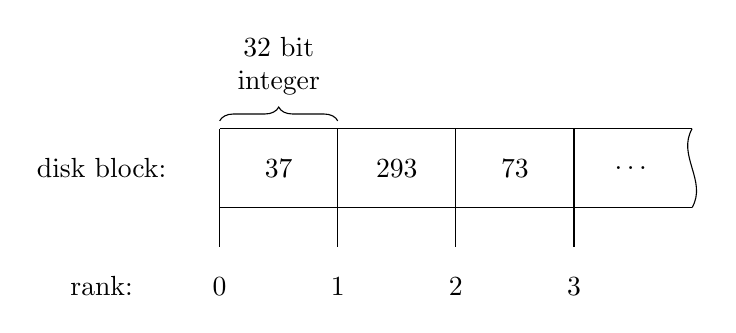
\begin{tikzpicture}[node distance={15mm}, main/.style = {draw, circle}]

    \draw (0,0) -- (6,0);
    \draw (0,1) -- (6,1);
    \draw (0,-0.5) -- (0,1);
    \draw (1.5,-0.5) -- (1.5,1);
    \draw (3,-0.5) -- (3,1);
    \draw (4.5,-0.5) -- (4.5,1);
    \draw[out=60, in=-120] (6,0) to (6,1);

    \node at (0.75, 0.5) {37};
    \node at (2.25, 0.5) {293};
    \node at (3.75, 0.5) {73};
    \node at (5.25, 0.5) {…};

    \node at (-1.5, 0.5) {disk block:};
    \node at (-1.5, -1) {rank:};
    \node at (0, -1) {0};
    \node at (1.5, -1) {1};
    \node at (3, -1) {2};
    \node at (4.5, -1) {3};

    \draw [decorate,decoration = {brace, amplitude=5pt}] (0,1.1) --  (1.5,1.1);
    \node[ align=center] at (0.75, 1.8) {32 bit  \\ integer};

\end{tikzpicture}
    \caption{Position File}
    \label{fig:position_file}
\end{figure}

\section{Reading Disk Arcs}

If one wants to get all upwards arcs of rank $i$ one needs take  the upwards position file, retrieve the integer $j$ that is stored at index $i$, and then read the complete block $j$ in the upwards arc file. 
There one will get an array, contain the requested arcs but also some other. These arcs are likely to be request next. Therefore we want to keep them in memory. We implemented two buffer a \textit{circular buffer} and a \textit{least recently used buffer} LRU

\subsection{Circular Buffer}

For the circular buffer we simply used an array of disk arcs. If we reach the end of the buffer we restart overwriting the values from the array start. To get the all arcs of a rank one request that rank number. There is a position hash table which tells the start position of that rank inside the buffer. If it is missing, the containing disk block is read to the buffer. It 
continues to read sequentially until the request rank and the read arc doesn't belong together anymore. This buffer has the advantage that we can exactly determine the amount of arcs we buffering. Also as it is just a simple array, it will be easy for the operation system to cache it.
The disadvantage is that it is possible that we request arc sets very often as it is possible they get evicted just before request again.

\subsection{Least Recently Used Buffer}

Cache is a \textit{java.util.LinkedHashMap}. This class provides the possibility to evicted the entry that has been requested longest time ago. In our case it maps ranks to sets of disk arcs. We can only determine how many 
disk arc sets we have in memory and disk arc sets do not have always the same size. Higher rank vertex usually have bigger sets as they are of higher degree. The advantage is, it is very easy to implement and therefore very 
resilient to programming errors.

\section{The Search}

The search brings all things explained in this chapter together. 

At the beginning there are to index graphs initialized the upwards graph $G_\uparrow'(V_\uparrow, A_\uparrow)$ and the downwards graph $G_\downarrow'(V_\downarrow, A_\downarrow)$. We are looking for the shortest
path from the source vertex $v(s)$ to the target vertex $v(t)$. The vertex set $V_\uparrow$ of the upwards graph $G_\uparrow'(V, A_\uparrow)$ only contains one vertex $v(s)$ and the $A_\uparrow$ only contains 
the upward edges to $v(s)$. The vertex set $V_\downarrow$ of the downwards graph $G_\downarrow'(V_\downarrow, A_\downarrow)$ only contains the $v(t)$ and the edge set $A_\downarrow$ only contain the arcs to $v(t)$.
\\
Now both $G_\uparrow'$ and $G_\uparrow'$ are alternatingly expanded with CH-Dijkstra. When the CH-Dijkstra has decided which vertex to expand next, the buffer will be requested to load its neighborhood. This can be 
compared to Command \& Conquer or a lot of other strategy  real-time strategy video games where you start at a map that is almost completely grey and the map is only load to the position you are plus some padding.
The rest is just a plain CH-Search where we stop after we determined the correct shortest path.

%\begin{figure}
%    \centering
%    \begin{tikzpicture}[node distance={15mm}, main/.style = {draw, circle}]

    \draw (0,0) -- (9,0);
    \draw (0,1) -- (9,1);
    \draw (0,-0.5) -- (0,1);
    \draw (1.5,-0.5) -- (1.5,1);
    \draw (3,-0.5) -- (3,1);
    \draw (4.5,-0.5) -- (4.5,1);
    \draw (6,-0.5) -- (6,1);
    \draw (7.5,-0.5) -- (7.5,1);
    \draw (9,-0.5) -- (9,1);

    \node<2-4> at (0.75, 0.5) {a(1,x)};
    \node<2-4> at (2.25, 0.5) {a(1,y)};
    \node<2-4> at (3.75, 0.5) {a(1,z)};
    \node<5-> at (0.75, 0.5) {a(3,x)};
    \node<5-> at (2.25, 0.5) {a(3,y)};
    \node<5-> at (3.75, 0.5) {a(3,z)};
    \node<3-4> at (5.25, 0.5) {a(2,x)};
    \node<5-> at (5.25, 0.5) {a(3,zx)};
    \node<3-> at (6.75, 0.5) {a(2,y)};
    \node<3-> at (8.25, 0.5) {a(2,z)};

    \node at (-1.5, 0.5) {DiskArc[]};
    \node at (-1.5, -1) {index:};
    \node at (0, -1) {0};
    \node at (1.5, -1) {1};
    \node at (3, -1) {2};
    \node at (4.5, -1) {3};
    \node at (6, -1) {4};
    \node at (7.5, -1) {5};
    \node at (9, -1) {size};

    \draw<1>[ -Stealth, ] (0, -4 ) -- node[above, sloped] {writePointer} (0,-1.5);
    \draw<2>[ -Stealth, ] (4.5, -4 ) -- node[above, sloped] {writePointer} (4.5,-1.5);
    \draw<3-4>[ -Stealth, ] (0, -4 ) -- node[above, sloped] {writePointer} (0,-1.5);
    \draw<5-6>[ -Stealth, ] (6, -4 ) -- node[above, sloped] {writePointer} (6,-1.5);



    \node at (-1.5, 2) {positions:};
    \onslide<1>{\node (tab1)  at (3,2) {%
        \begin{tabular}{c }
            \textbf{rank} \\
            \hline
            \textbf{position} \\
        \end{tabular}};
    }
    \onslide<2>{\node (tab1)  at (3,2) {%
        \begin{tabular}{c | c }
            \textbf{rank} & 1  \\
            \hline
            \textbf{position} & 2  \\
        \end{tabular}};
    }
    \onslide<3>{\node (tab1)  at (3,2) {%
        \begin{tabular}{c | c | c }
            \textbf{rank} & 1 & 2 \\
            \hline
            \textbf{position} & 2 & 5 \\
        \end{tabular}};
    }
    \onslide<4>{\node (tab1)  at (3,2) {%
        \begin{tabular}{c | c | c | c}
            \textbf{rank} & 1 & 2 & max(rank) \\
            \hline
            \textbf{position} & 2 & 5 & -1 \\
        \end{tabular}};
    }
    \onslide<5>{\node (tab1)  at (3,2) {%
        \begin{tabular}{c | c | c | c | c}
            \textbf{rank} & 1 & \textcolor{red}{2} & 3 & max(rank) \\
            \hline
            \textbf{position} & 2 & \textcolor{red}{5} & 3 & -1 \\
        \end{tabular}};
    }
    \onslide<6->{\node (tab1)  at (3,2) {%
        \begin{tabular}{c | c | c | c }
            \textbf{rank} & 1 & 3 & max(rank) \\
            \hline
            \textbf{position} & 2 & 3 & -1 \\
        \end{tabular}};
    }

    \onslide<5>{
      \node at (0,-2){\textcolor{red}{remove incomplete edge set from position}};
    }
   

\end{tikzpicture}
%    \caption{Circular Buffer}
%    \label{fig:circular_buffer}
%\end{figure}
